\chapter{Análise de Resultados} \label{ch:analise_resultados}

Este capítulo apresenta a análise dos resultados obtidos a partir do desenvolvimento da linguagem proposta, organizados com relação aos objetivos específicos estabelecidos na \autoref{sec:objetivos}. Ele está dividido em três seções, incluindo a análise geral da implementação, as decisões de desenvolvimento e seus impactos, e por fim, a viabilidade e limitações da solução proposta, determinando se os objetivos do trabalho foram alcançados.

\section{Análise Geral da Implementação da Solução}

A implementação do protótipo de interpretador para a linguagem proposta se mostrou muito parecida com a implementação de interpretadores de linguagens tradicionais. Isso se deve ao fato dele possuir todas as fases genéricas de um interpretador tradicional implementadas, já que foi feito com base na primeira metade do livro \textit{Crafting Interpreters}, e consequentemente feito com base em Jlox \cite{craftinginterpreters}.

Saindo do escopo de fases de um interpretador e indo mais a fundo na implementação, também foi possível observar semelhanças de sintaxe com linguagens tradicionais. Um exemplo disso é a sintaxe de declaração de sistemas, que é muito parecida com a sintaxe de declaração de funções em Jlox, Rust, e muitas outras linguagens \cite{rustbook,craftinginterpreters}.

Usando regras de produção, a figura \ref{fig:decl_sistema_funcao} demonstra a semelhança entre a sintaxe de declaração de sistemas na linguagem proposta e a sintaxe de declaração de funções em Jlox. Nota-se que há apenas duas diferenças: a palavra-chave \texttt{system} no lugar de \texttt{fun} e a sintaxe de \textit{query} no lugar da lista de parâmetros.

\begin{figure}[H]
	\centering
	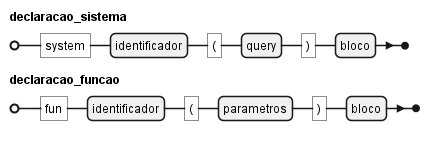
\includegraphics[width=0.45\textheight]{../diagrams/decl_sistema_funcao.png}
	\caption{Diagrama de sintaxe comparando declaração de sistemas e de funções.}
	\fonte{Elaboração própria com PlantUML feita com base no interpretador nosso e no de Jlox \cite{craftinginterpreters}.}
	\label{fig:decl_sistema_funcao}
\end{figure}

Vale ressaltar que semelhanças como essa estão presentes em outras partes da sintaxe da linguagem proposta, e foram intencionalmente feitas para facilitar a legibilidade e a facilidade de escrita através da familiaridade com outras linguagens, conforme discutido na \autoref{sec:design_linguagem}.

Fora as semelhanças, as diferenças na implementação da linguagem proposta foram encontradas principalmente na semântica e na pragmática \cite{designconceptsinlanguages}, que foram adaptadas para suportar os conceitos de ECS.

Ainda no exemplo de declaração de sistemas, a semântica foi feita de forma que o interpretador reconheça um sistema como uma função que atua sobre entidades e seus componentes de forma automática. Já a pragmática foi feita através da ligação da sua sintaxe com a API da biblioteca de ECS Flecs.

A fim de melhor documentar o processo de desenvolvimento da implementação, a seção seguinte detalha as principais decisões feitas durante o desenvolvimento do interpretador.

\section{Decisões de Desenvolvimento e seus Impactos}

Esta seção tem a finalidade de documentar as principais decisões tomadas durante o desenvolvimento do interpretador em um só lugar, possivelmente servindo de referência para trabalhos futuros. Para cada decisão, será descrito o objetivo da decisão, a decisão em si, seu impacto no protótipo, e, caso aplicável, alternativas relevantes.

\subsection{Escolha da Linguagem de Implementação}

\begin{itemize}
	\item \textbf{Objetivo}: Escolher uma linguagem de programação adequada para implementar o interpretador, considerando fatores como suporte de bibliotecas, estruturas de dados expressivas e familiaridade do desenvolvedor;
	\item \textbf{Decisão}: A linguagem escolhida foi Rust, devido ao seu suporte a \textit{Algebraic Data Types} através de \texttt{enums} \cite{rustbook}, seu ecosistema com as bibliotecas necessárias, e a familiaridade do desenvolvedor com a linguagem;
	\item \textbf{Impacto}: A escolha de Rust tornou o processo de depuração extremamente previsível devido ao seu sistema de tipos rígido, além de permitir abstrações mais expressivas através de \texttt{enums} \cite{rustbook}. Porém, devido a sua tipagem estática, a implementação da ponte entre o interpretador e a biblioteca de ECS exigiu uma estratégia incomum \cite{rustbook}. % TODO! Referenciar a estratégia incomum quando ela for implementada.
\end{itemize}

\subsection{Escolhas de \textit{Design} da Linguagem}

\begin{itemize}
	\item \textbf{Objetivo}:
	\item \textbf{Decisão}:
	\item \textbf{Impacto}:
\end{itemize}

\subsection{Representação das Abstrações Internas}

\begin{itemize}
	\item \textbf{Objetivo}:
	\item \textbf{Decisão}:
	\item \textbf{Impacto}:
\end{itemize}

\subsection{Estratégia de Análise Léxica}

\begin{itemize}
	\item \textbf{Objetivo}:
	\item \textbf{Decisão}:
	\item \textbf{Impacto}:
\end{itemize}

\subsection{Estratégia de Análise Sintática}

\begin{itemize}
	\item \textbf{Objetivo}:
	\item \textbf{Decisão}:
	\item \textbf{Impacto}:
\end{itemize}

\subsection{Estratégia de Interpretação}

\begin{itemize}
	\item \textbf{Objetivo}:
	\item \textbf{Decisão}:
	\item \textbf{Impacto}:
\end{itemize}

\subsection{Escolha da Biblioteca de ECS}

\begin{itemize}
	\item \textbf{Objetivo}:
	\item \textbf{Decisão}:
	\item \textbf{Impacto}:
\end{itemize}

\subsection{Representação Interna de Entidades, Componentes e Sistemas}

\begin{itemize}
	\item \textbf{Objetivo}:
	\item \textbf{Decisão}:
	\item \textbf{Impacto}:
\end{itemize}

\section{Viabilidade e Limitações da Solução}
